\documentclass{article}

\usepackage{amssymb}
\usepackage{amsmath}
\usepackage{graphicx}
\usepackage{mathptmx}
\usepackage{lipsum}  % for sample text
\usepackage[T1]{fontenc}
\usepackage{textcomp}
\usepackage{dirtytalk}
\usepackage{listings}
% \usepackage{subfigure}
\usepackage{subcaption}


%include these lines if you want to use the LaTeX "theorem" environments
\newtheorem{theorem}{Theorem}[section]
\newtheorem{definition}[theorem]{Definition}
\newtheorem{lemma}[theorem]{Lemma}
\newtheorem{corollary}[theorem]{Corollary}


%include lines like this if you want to define your own commands 
%to save typing
\newcommand{\PROOF}{\noindent {\bf Proof}: }
\newcommand{\REF}[1]{[\ref{#1}]}
\newcommand{\Ref}[1]{(\ref{#1})}
\newcommand{\dt}{\mbox{\rm   dt}}
\newcommand{\phat}{\hat{p}}


 \usepackage{setspace}
 \onehalfspacing
 \newtheorem{mytheorem}{Theorem}
 \numberwithin{mytheorem}{subsection} % important bit


\begin{document}

	\title{Mini Paper: The Penney Ante Problem}
	\author{Saleh Hindi}

	\maketitle

	\section{Introduction}
		Imagine a two player game where
		each player is assigned a sequence, for example THTH and HTHH, and a coin is flipped until either player sees their sequence.
		The first player to see their sequence appear wins.
		Given two sequences, which sequence is expected to come first in the
		sequence of coin flips? What is the probability of a certain player winning? Although these two
		questions sound similar, the result is that in our example,
		the expected number of turns for sequence A to appear is 20 and for B it is 18. Meanwhile, the probability
		of A winning is 9/14 while the probability of B winning is 5/14. Additionally the game has the property
		that for any sequence A chooses, B can always find a sequence that has a higher probability of winning.
		These counterintuitive results are the core of the Penney Ante problem, discovered by Walter Penney
		\cite{gardner}. My thesis will study this problem through three approaches based in Markov chains, martingales,
		and a combinatoric approach.

	\section{Definitions and Notation}
		Let $X_t$ be a random variable for $t \geq 1$, and let $(X_t)$ be a stochastic sequence of letters chosen uniformly and
		randomly from a $q$-letter alphabet. In our case, $q=2$ and $(X_t)$ represents the sequence of coin flips. Let $A=a_1a_2a_3...$ and $B=b_1b_2b_3...$ be sequences
		of $n$ letters chosen from the $q$-letter alphabet. We say
		sequence $A$ or $B$ wins if it is the first sequence to appear within $(X_t)$. Let $\tau_A$ and $\tau_B$ be random variables denoting
		the number of turns for $A$ or $B$ to appear. We denote
		the probability of $A$ winning as $P(\tau_A < \tau_B)$ and we denote the expected time for sequence
		$A$ and $B$ to appear as $E(\tau_A)$ and $E(\tau_B)$.

		As stated earlier, $E(\tau_A) < E(\tau_B)$ does not imply $P(\tau_A < \tau_B) > \frac{1}{2}$. To prove and understand this result, we will be using 
		a mathematical object called Markov chains which has the probability that each state occuring, ie each $X_k$, is based solely on $X_{k-1}$ for all $k > 1$. Markov chains imagine the game as a graph with vertices representing (Be precise about this. Each state represents how close you are to winning right? I should define this thing here) some subset of $(X_t)$ and edges denoting probabilities between edges. More formally,

		\begin{definition}[\cite{textbook}]
			XXXNote that Xk is not an event, is a single random variableXXX A Markov chain is a stochastic sequence such that
			$$P(X_{k+1} = x | X_1X_2...X_k) = P(X_{k+1} = x  | X_k)$$
			That is, the probability that an event occurs given the entire history of
			previous events is only dependent on the most recent event. Denote the probability
			that event $y$ occurs given $x$ as $P(x,y)$.
		\end{definition}

		The Penney ante game is a Markov chain because each coin flip $X_k$ is chosen uniformly and randomly from the set of possible coin flips so it does not depend on.... It's because each vertex is an event like HHT and this is only dependent on the previous event. We can use Markov chains to find $E(\tau_A)$ and $P(\tau_A < \tau_B)$ by modelling each X if for 1 <= i <= n as a systems of equations which will be done next section. 

		We can also study the Penney ante problem using another mathematical object called a martingale. Let $\tau$ be any betting strategy on $(X_t)$ and let $W_t$ be the earnings until time $t$ (define a betting strategy). A martingale is a game such that regardless of the betting strategy, the expected earnings is the same at any time. A martingale with an expected earnings of 0 is called a fair game. More precisely,   

		\begin{definition}[\cite{li}]
			(Is this correct?) A martingale is a stochastic sequence $(X_t)$ such that for any
			integer $k$ and for any finite expected value $E(|X_k|)$, $$E(X_{k+1} | X_1, ..., X_k) = X_k$$		
		\end{definition}

		(How do I know this game is a martingale?) Let's define a betting strategy on the game. At each time, a new player enters the game and bets 1 on $X_t$ being $a_t$. The player bets double or nothing on each subsequent coin flip. If any of the players lose at any point, they stop betting. Given two sequences A and B, define the operation AB as the total earnings of the players if they bet on B given A occurs (check this). Conway devised a "magic algorithm" which let us computer AB which will be used to find the expected winning time and the probability of A winning.

		And finally, we will be using a combinatoric method for finding $E(\tau_A)$ based around finding the generative function for XXX. A generative function is a function for counting the number of strings such that it contains no occurences of a given string as a substring. 
		\begin{definition}[\cite{}]

		Finally, we define nontransitivity. In this context, a game is nontransitive if for any sequence A, player B can choose a sequence B such that $P(\tau_A < \tau_B)$. In later sections we will see that the Penney ante game is nontransitive for $n > 4$. In general nontransitivity is....

	\section{Results}
		Using Markov chains, we can construct a system of equations for the expected value and probability. Let $p_{x}$ denote the probability of A winning given that $x$ has occured. To find $p_\emptyset$, the probability of A winning given nothing has happened, we can construct a system of $|\Omega|$ equations for each $x \in \Omega$ composed of the sum of the possible ways to reach $x$ times their probabilities times the probability of reaching $x$ from $y$.

		% \textasciitilde for a tilde
		$$p_x = \sum_{y - x} P(x,y) p_y$$

		In this game, for a $q=2$ alphabet each sum will have two terms since there will only be at most two states $x$ that are reachable from each state $y$. Similarly, we can find the expected value this method but with a small change. Let $E_x$ denote the time to win given $x$ has occurred. Then we can write a system of $|\Omega|$ equations for each $x \in \Omega$,

		$$E_x = \sum_{y - x} P(x,y) (1 + E_y)$$

		Note the we add 1 to $E_y$ because.... 

		For when thinking about the Penney ante problem in terms of martingales, we can use Conway's algorithm to find $P(\tau_A < \tau_B)$ and $E(\tau_A)$. Conway devised an algorithm for computing these two values which has been described as an algorithm that "cranks out the answer as if by magic" \cite{gardner}. The algorithm is as follows,

		\begin{theorem}(Conway's Algorithm \cite{gardner})
		Given two n-tuples A and B, we find the binary representation of
		the operation $A \oplus B$ by the following algorithm:
		\begin{enumerate}
		\item loop through integers 1, 2, ..., n,
		\item At every ith iteration we look at the ith through nth digits of A and compare
		   it to the 1st through the (n-i)th digits of B.
		\item If these subsequences are equal, the ith digit in the binary representation is 1 but 0 otherwise.
		\end{enumerate} 

		The binary representation of $A \oplus B$
		is then converted to a decimal number. Once we find $A \oplus A$, $A \oplus B$,
		$B \oplus A$, and $B \oplus B$, the probability that A precedes B is
		$$P(\tau_A < \tau_B) = \frac{A \oplus A - A \oplus B}{(B \oplus B - B \oplus A) + (A \oplus A - A \oplus B)} $$
		Furthermore, 
		$$E(\tau_A) = 2 (A\oplus A) $$ 

		Consider $THTH \oplus THTH$ as an example.  
		\begin{lstlisting}[escapechar=\%]
		1010 
		%\underline{THTH}%
		THTH
		 THTH
		  THTH 
		   THTH 
		\end{lstlisting}

		The binary number 1010 in decimal is 9 so $E(\tau_{THTH}) = 18$.

		\end{theorem}

		Using the generative approach, we find that ....


	\section{Examples}
		\begin{figure}
		\centering
		\begin{minipage}{.3\textwidth}
		  \centering
		  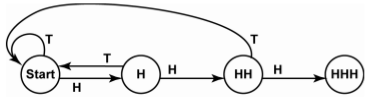
\includegraphics[width=1.0\linewidth]{StateDiagramforHHH}
		  \captionof{figure}{The graph of $\Omega_A$}
		  \label{fig:test1}
		\end{minipage}%
		\begin{minipage}{.3\textwidth}
		  \centering
		  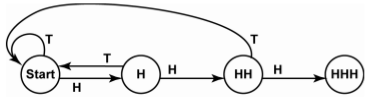
\includegraphics[width=1.0\linewidth]{StateDiagramforHHH}
		  \captionof{figure}{The graph of $\Omega_B$}
		  \label{fig:test2}
		\end{minipage}
		\begin{minipage}{.3\textwidth}
		  \centering
		  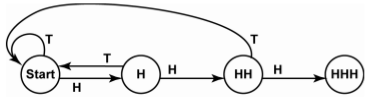
\includegraphics[width=1.0\linewidth]{StateDiagramforHHH}
		  \captionof{figure}{Another figure}
		  \label{fig:test2}
		\end{minipage}
		\end{figure}

		As an example, let $A = THTH$ and $B = HTHH$. Although not all possible sequences have the property that, $E(\tau_A) < E(\tau_B)$ while $P(\tau_A < \tau_B) > \frac{1}{2}$, these two do so it is a worthwhile example to consider. (Could there be any other good examples? Maybe for a dice?) As stated in the introduction, $E(\tau_A)$ is 20, $E(\tau_B)$ is 18, and $P(\tau_A > \tau_B) = \frac{9}{14}$. As a sanity check, we should check that the three methods described in the previous section give the same answer for $P(\tau_A > \tau_B)$ and $E(\tau_B)$. For $\Omega$, $\Omega = n^q$ which is 16 in this case (this is wrong because we only count states that get us closer to A). Here are a couple of equations as an example with the Mathematica code to solve the equations (How should I work through this long example? Should I show all equations). For the probability we have,

		\begin{equation} 	
		\begin{split}
		p_{\emptyset} & = \frac{1}{2} XX + \frac{1}{2} XX \\
		p_{T} & = \frac{1}{2} XX + \frac{1}{2} XX \\
		p_{TH} & = \frac{1}{2} XX + \frac{1}{2} XX \\
		p_{THT} & = \frac{1}{2} XX + \frac{1}{2} XX \\
		p_{THTH} & = 1 \\
		\end{split}
		\end{equation}


		Using Mathematica we find that $p_{THTH} = \frac{9}{14}$. For the expected value we have,

		\begin{equation} 	
		\begin{split}
		E_{\emptyset} & = \frac{1}{2} (1 + XX) + \frac{1}{2} (1 + XX) \\
		E_{T} & = \frac{1}{2} (1 + XX) + \frac{1}{2} (1 + XX) \\
		E_{TH} & = \frac{1}{2} (1 + XX) + \frac{1}{2} (1 + XX) \\
		E_{THT} & = \frac{1}{2} (1 + XX) + \frac{1}{2} (1 + XX) \\
		E_{THTH} & = \frac{1}{2} (1 + XX) + \frac{1}{2} (1 + XX) \\
		\end{split}
		\end{equation}

		The calculation for B is omitted because it is essentially the same. Using the same Mathematica code we find that $E_{THTHT} = 20$.


	\section{Connection Between Techniques}
		Blah

	\section{Future Work}
		In the future I will prove the results stated in the results section. It will also be worthwhile to give a proof of the nontransitivity property which was not stated in the results.

	\begin{thebibliography}{1}
		\bibitem{boyer}
			Boyer, Robert S., and J. Strother Moore. "A Fast String Searching Algorithm." Communications of the ACM 20.10 (1977): 762-72. Web. 
		\bibitem{breen}
			Breen, Stephen, Waterman Michael S., and Zhang Ning. "Renewal Theory for Several Patterns." Journal of Applied Probability 22.1 (1985): 228-34. Web.
		\bibitem{gardner}
			Gardner, Martin. "Mathematical Games: On the Paradoxical Situations That Arise from Nontransitive Relations." Scientific American 10 (1974): 120-25. Print.
		\bibitem{guibas}
			Guibas, L.j, and A.m Odlyzko. "String Overlaps, Pattern Matching, and Nontransitive Games." Journal of Combinatorial Theory, Series A 30.2 (1981): 183-208. Web.
		\bibitem{li}
			Li, Shuo-Yen Robert. "A Martingale Approach to the Study of Occurrence of Sequence Patterns in Repeated Experiments." The Annals of Probability 8.6 (1980): 1171-176. Web.
		\bibitem{nickerson}
			Nickerson, R. S. "Penney Ante: Counterintuitive Probabilities in Coin Tossing." The UMAP Journal 28.4 (2007): 503-32. JSTOR. Web. 8 Sept. 2016. 
		\bibitem{textbook}
			Levin, David Asher, Y. Peres, and Elizabeth L. Wilmer. Markov Chains and Mixing times. Providence, RI: American Mathematical Society, 2009. Print. 
		\bibitem{enumerate}
			FILL IN LATER for Enumeration of Strings
			
	\end{thebibliography}
\end{document}

 